\documentclass[12pt]{article}
\usepackage{amssymb,mathrsfs, amsmath,amsfonts}
\usepackage{mathtools}
\usepackage{graphicx}
\usepackage{enumitem}
\usepackage{braket}
\graphicspath{ {./ps6-assets/}{./exercises/handwritten/ps6/ps6-assets/} }

\title{Problem Set 6 Solutions}
\author{CSE 468}
\date{\today}

\begin{document}

\maketitle

\begin{enumerate}[font=\bfseries]
    \item \begin{enumerate}
        \item In both cases the state of the bottom qubit is $\ket{-}$. Suppose $f(0) = f(1) = 0$.
        \[\ket{\psi_2} = \ket{+} \otimes (\ket{0} - \ket{1}) = \ket{+-}\]
        Similarly obtained for $f(0) = f(1) = 1$. Don't forget to ignore global phase.
        Now suppose $f(0) = 0, f(1) = 1$.
        \[\ket{\psi_2} = \ket{-} \otimes (\ket{0} - \ket{1}) = \ket{--}\]
        Similarly obtained for $f(0) = 1, f(1) = 0$. Don't forget to ignore global phase.
        \item 50\% time see $\ket{0}$ and 50\% time see $\ket{1}$
        \item $\ket{1}$
    \end{enumerate}
    \item \begin{enumerate}
        \item $k = 0.5$
    \item 
    Some helpful hints from Lecture 23:
    \[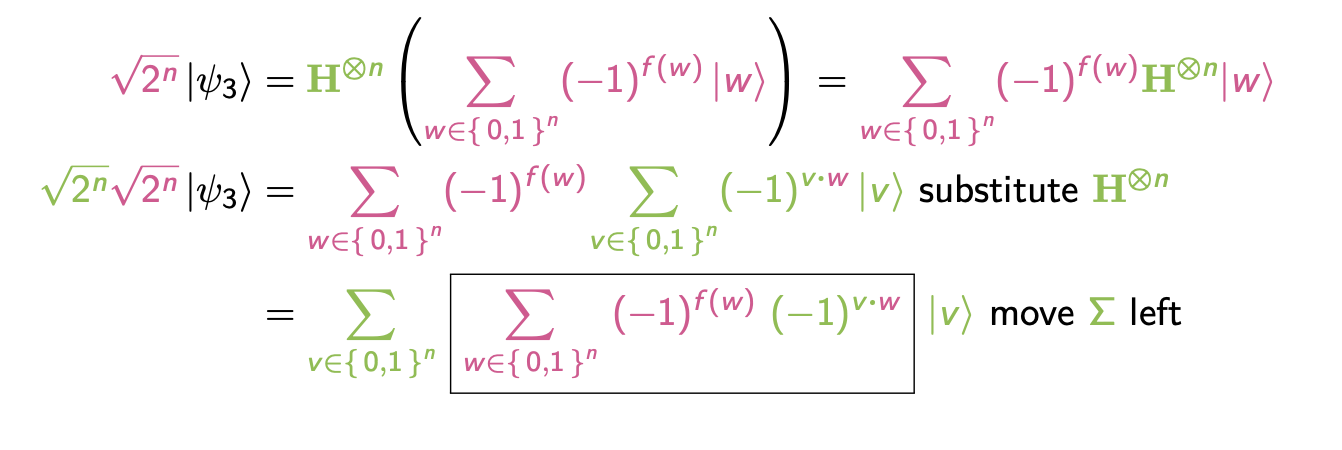
\includegraphics[scale=0.6]{ps6_hint1}\]
    \[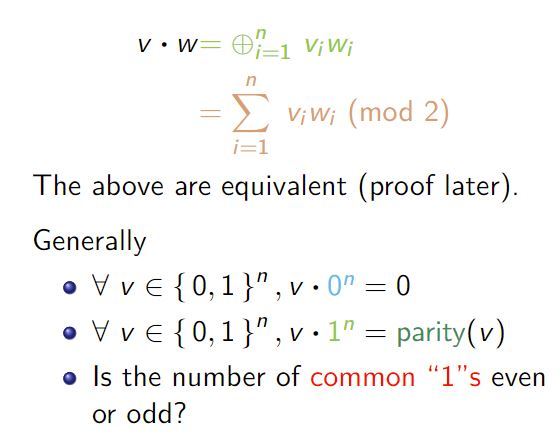
\includegraphics[scale=0.6]{ps6_hint2}\]
    \begin{itemize}
        \item $\ket{00}$ has amplitude $-\frac{1}{2}$
        \item $\ket{01}$ has amplitude $\frac{1}{2}$
        \item $\ket{10}$ has amplitude $\frac{1}{2}$
        \item $\ket{11}$ has amplitude $\frac{1}{2}$
    \end{itemize}
    \item $(\frac{1}{2})^2 = \frac{1}{4}$. Probability = amplitude squared. 
    \item $1 - \frac{1}{4} = \frac{3}{4}$
    \item 
    \end{enumerate}
\end{enumerate}



\end{document}